\documentclass[serif]{beamer} % use draft mode for speed !
\usepackage{pacman}
\usepackage[english]{babel}
\usepackage[utf8]{inputenc}
\usepackage{amsmath, amsfonts, wasysym}
\usepackage{listings}
\usepackage{tikz}
\usetikzlibrary{positioning}
\usetikzlibrary{arrows}
\usetikzlibrary{calc}
\usetikzlibrary{backgrounds}
\usetikzlibrary{trees}
\usetikzlibrary{shadows}

\author[Joël Falcou]{Serge Guelton, Pierrick brunet, \textbf{Joël Faclou}}

\title[\texttt{pythran}]{Exploring the Vectorization of Python Constructs Using Pythran and Boost SIMD}

\date{30 janvier 2014}

\institute{QuarksLab / INRIA / LRI}

\tikzstyle{every picture}+=[remember picture]

\begin{document}

\begin{frame}
\maketitle
\end{frame}

\section{Motivation}
\begin{frame}{Why Python?}

  \begin{itemize}
      \item High level language $\rightarrow$ many abstractions, nice $\frac{\textsc{SLOC}}{\text{heure}}$
      \item Rich Ecosystem $\rightarrow$ favor reuse
      \item Dynamic typing $\rightarrow$ $\simeq$\structure{Structural Typing}
      \item Built-in containers: \texttt{list}, \texttt{set}, \texttt{dict}
      \item Scientific modules: \texttt{scipy}, \structure{\texttt{numpy}}
  \end{itemize}
  \begin{center}
	\structure{Nice for fast prototyping}
  \end{center}
  \begin{center}
	\alert{But\dots}
  \end{center}
  \begin{itemize}
      \item interpreted, dynamic code is slow (\frownie late binding)
      \item no fine grain parallelism (ugly \textsc{gil})
  \end{itemize}

\end{frame}

\begin{frame}{How to get fast}
  \begin{block}{Use native code}
      Python has built-in support for writing native modules
  \end{block}

  \begin{block}{Beware!}
      Conversion cost from sparse to dense structures
  \end{block}
  \begin{center}
      Find Hotspots, turn them into native, parallel, \structure{vectorized} native functions
  \end{center}
\end{frame}

\begin{frame}{What we're interested in}
  \begin{center}
  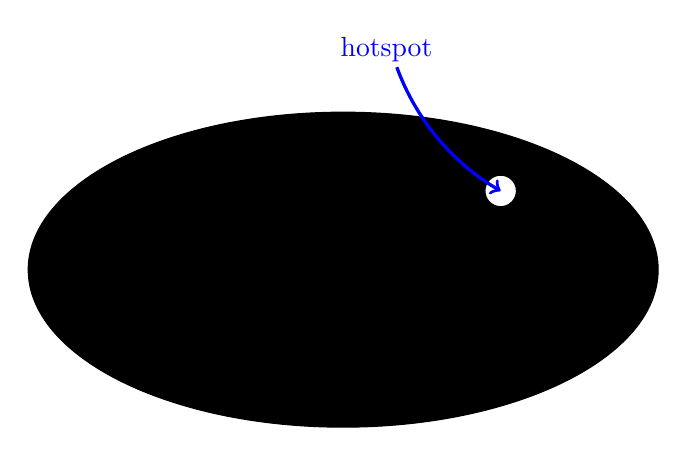
\begin{tikzpicture}
	\draw[fill=black] (0,0) ellipse (4 and 2);
	\draw[fill=white] (2,1) circle (.2);
	\draw[draw=blue,very thick,<-] (2,1) arc (60:20:-3); 
	\node[text=blue] at (.55,2.8) {hotspot};
  \end{tikzpicture}

  \structure{Challenge} write everything in Python, use a compiler to speedup the \color{blue}{hotspot}\end{center}
\end{frame}

\begin{frame}[allowframebreaks=.9]{Existing solutions}
    \begin{block}{Just In Time Compilers}
        \begin{description}
            \item[PyPy] generic, the holy grail
            \item[Parakeet] Numpy \& performance centric
            \item[Numba] Numpy centric, LLVM-based
            \item[Copperhead] functional style!
        \end{description}
    \end{block}

    \begin{block}{Ahead of Time Compilers}
        \begin{description}
            \item[Nuitka] Not performance-centric
            \item[Shedskin] No parallelism
            \item[Pythran] Parallelization through OpenMP and Boost.SIMD
        \end{description}
    \end{block}

\end{frame}

\begin{frame}{Compilation Flow}
  \scalebox{.9}{
  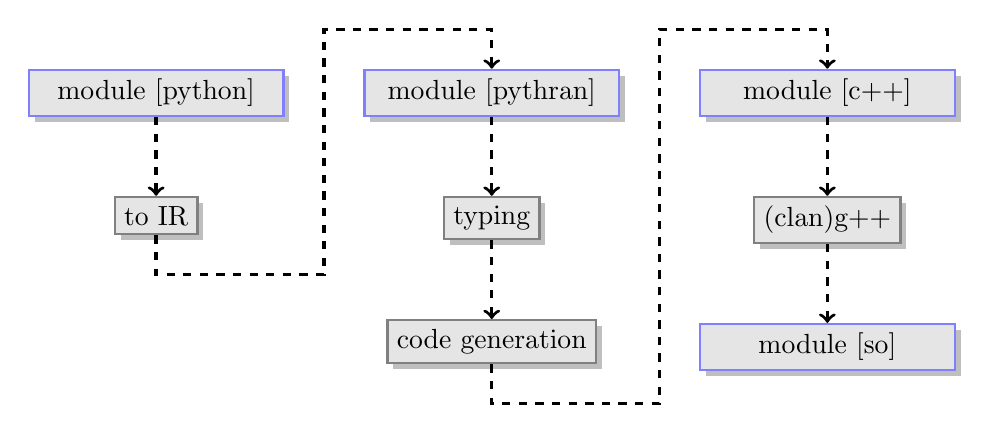
\begin{tikzpicture}[pass/.style={rectangle,draw=black!50,fill=black!10,thick,drop
	shadow,align=center},
	obj/.style={rectangle,draw=blue!50,fill=black!10,thick,drop	shadow,text width=3cm, align=center}]
	\node[obj] (python) {module [python]};
	\node[pass] (ast-refine) [below=of python] {to IR};
	\node[obj] (pythran) [right=of python] {module [pythran]};
	\node[pass] (typing) [below=of pythran]{ typing};
	\node[pass] (backend)[below=of typing] { code generation};
	\node[obj] (cxx) [right=of pythran] {module [c++]};
    \node[pass] (rbackend) [below=of cxx] { (clan)g++};
	\node[obj] (so) [below=of rbackend] {module [so]};

	\draw[->, very thick, dashed] (python) -- (ast-refine);
	\draw[->, very thick, dashed] (ast-refine.south) |- ($(ast-refine.south) - (0,0.5)$) -| ($.5*(python.east) + .5*(pythran.west)$) |- ($(pythran.north) + (0,0.5)$) -| (pythran);

	\draw[->, very thick, dashed] (pythran) -- (typing);
	\draw[->, very thick, dashed] (typing) -- (backend);
	\draw[->, very thick, dashed] (backend.south) |- ($(backend.south) - (0,0.5)$) -| ($.5*(pythran.east) + .5*(cxx.west)$) |- ($(cxx.north) + (0,0.5)$) -| (cxx);

	\draw[->, very thick, dashed] (cxx) -- (rbackend);
	\draw[->, very thick, dashed] (rbackend) -- (so);
  \end{tikzpicture}
  }
\end{frame}

\begin{frame}{TOC}
  \tableofcontents
\end{frame}

\section{Python, typing and animals}

\subsection{typing functions}
\begin{frame}[fragile]{Python, functions and C++11}
  \begin{block}{Typing in Python}
      structural typing, a.k.a. \emph{duck typing}
  \end{block}
  \uncover<1-2>{
  \begin{center}
	\only<1>{\scalebox{5}{\lstinputlisting[basicstyle=\scriptsize\ttfamily]{duck.txt}}}
	\only<2>{\scalebox{.6}{\lstinputlisting[basicstyle=\scriptsize\ttfamily]{dragon.txt}}}
  \end{center}
  }
  \uncover<3>{
  \begin{block}{Tying in C++}
	nominal typing, \texttt{Duck != Dragon}\\
	\alert{but}~: structural typing \emph{using} meta programing!
	\lstinputlisting[basicstyle=\scriptsize\ttfamily,language=c++]{cxx_sample_template.cpp}
  \end{block}
  \alert{Easy way to support polymorphic functions in C++}
  }

\end{frame}

\begin{frame}[fragile]{Example}
\begin{lstlisting}[basicstyle=\scriptsize\ttfamily,language=c++,]
struct f
{
  template<class T>
  auto operator()(T const& p)
  -> decltype(p * p)
  {
    return p * p;
  }
};
\end{lstlisting}

\structure{\hrule}\hspace{1em}

Pythran provides a header-based runtime called \texttt{pythonic} that provides most of Python's intrinsics and a few modules, including \texttt{operator}, \texttt{math} and (part of) \texttt{numpy}
\end{frame}


\section{Toward implicit vectorization}

\begin{frame}[fragile]
    \frametitle{Where's Wally?}
    \centering
    \begin{lstlisting}[language=Python,escapechar=!]
a = map(!\tikz[remember picture,overlay]{\node (map) {};}!math.cos, l)
b = [!\tikz[remember picture,overlay]{\node (listcomp) {};}!abs(i) for i in l]
c = sum(!\tikz[remember picture,overlay]{\node (sum) {};}!l)
d = numpy.sin(!\tikz[remember picture,overlay]{\node (np-sum) {};}!e !\tikz[remember picture,overlay]{\node (np-add) [yshift=.2em] {\texttt{+}};}! 2 !\tikz[remember picture,overlay]{\node (np-mul) [yshift=.2em] {\texttt{*}};}! f)
\end{lstlisting}

    \uncover<2->{
\begin{itemize}
    \item Implicit loops \tikz[remember picture,overlay]{\node (loops) {};}

    \uncover<3->{
    \item Implicit reductions \tikz[remember picture,overlay]{\node (reduction) {};}
    }
\end{itemize}
    }

\only<2>{
\begin{tikzpicture}[remember picture,overlay,very thick]
    \path (loops) edge[->, bend right] (map.south);
    \path (loops) edge[->, bend right] (listcomp.south);
    \path (loops) edge[->, bend right] (np-add.south);
    \path (loops) edge[->, bend right] (np-mul.south);
\end{tikzpicture}
}
\only<3>{
\begin{tikzpicture}[remember picture,overlay,very thick]
    \path (reduction) edge[->, bend right] (sum.south);
    \path (reduction) edge[->, bend right] (np-sum.south);
\end{tikzpicture}
}

\end{frame}

\begin{frame}{Requirements}
    \begin{block}{Type oblivious vectorization}
        Nothing is known about types at code generation time
    \end{block}
    \begin{block}{Tangled code}
        neither g++ nor clang++ can vectorize the high level C++ code from \texttt{pythonic}
    \end{block}
        \centering
        \structure{$\Rightarrow$} handle vectorization at compile time
        \newline
        \structure{$\Rightarrow$} generate parametric vectorized code

\end{frame}

\begin{frame}{Booooooooooost SIMD}
    Cover me, Jack. Jack! Jack? Jaaaaaack 
\end{frame}

\begin{frame}{High Level Skeletons}
    Run Hans!
\end{frame}

\section{Experiments}

\begin{frame}[fragile]
    \frametitle{Euler Problem 6}
    \centering
            \begin{lstlisting}{language=Python}
#pythran export solve(int)
def solve(n):
  r = range(1, n)
  a = sum(r)
  return a * a - sum(i * i for i in r)
            \end{lstlisting}

        \includegraphics[width=.9\textwidth]{euler06}
\end{frame}

\begin{frame}[fragile]
    \frametitle{Sum, Norm}
    \centering
    \begin{columns}
        \column{.5\textwidth}{
            \begin{lstlisting}{language=Python}
numpy.sum(a)
            \end{lstlisting}
        \includegraphics[width=\textwidth]{sum}
    }
    \column{.5\textwidth}{
        \begin{lstlisting}{language=Python}
numpy.sum(a * a)
        \end{lstlisting}
        \includegraphics[width=\textwidth]{sum_square}
    }
     \end{columns}
\end{frame}

\begin{frame}[fragile]
    \frametitle{Complex numpy expression}
\begin{lstlisting}
#pythran export rosen(float[])
def rosen(x):
    t0 = 100 * (x[1:] - x[:-1] ** 2) ** 2
    t1 = (1 - x[:-1]) ** 2
    return np.sum(t0 + t1)
\end{lstlisting}
\includegraphics[width=.9\textwidth]{rosen.pdf}
\end{frame}
\begin{frame}[fragile]
    \frametitle{After lazyness analysis}
\includegraphics[width=.9\textwidth]{rosen_fs.pdf}

\structure{3.07ms $\rightarrow$ 2.88ms} by avoiding more temporaries
\end{frame}

\section{The enD}

\begin{frame}{Conclusion and Perspectives}
    \framesubtitle{Python \& Vectorization}
    \begin{block}{\smiley{} Great \smiley{}}
        \begin{itemize}
            \item many implicit loops
            \item low hanging fruits with numpy
            \item great synergy between duck typing and Boost.SIMD
        \end{itemize}
    \end{block}
    \begin{block}{\frownie{} But \frownie{}}
        \begin{itemize}
            \item Conversion costs Python $\leftrightarrow$ C(++)
            \item Python uses \alert{long} integers
            \item Numpy defaults to \alert{double precision} arrays
        \end{itemize}
    \end{block}
\end{frame}

\end{document}
% vim:spell spelllang=en
